
\begin{figure}[H]
    \centering
    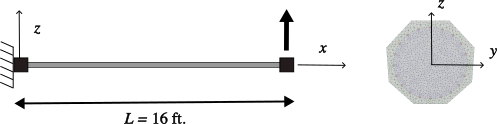
\includegraphics[width=0.6\linewidth]{Figures/column.png}
    \caption{Bridge column from the BRACE$^2$ project \citep{chern2024brace2}.}
    \label{fig:painter-column}
\end{figure}
An octagonal cantilever bridge column is subjected to an imposed transverse displacement. 
The multiaxial material of \cite{faria1998strainbased} is used to model the concrete. 

\FrameSection{
label/problem=frame-2021,
model=Fiber,
kinematics/section={\eqref{eq:linear-gl-strain-pi}},
shape=Octagon,
Iy=7.094e5,
Iz=7.094e5,
A=2982,
Ay=2553,
Az=2553,
J=1.396e6,
% Iyz=2.717e-11,
unit/length=\inch
}